\documentclass[runningheads]{llncs}
\usepackage{fontspec,xeCJK}
\setCJKmainfont{Noto Serif CJK SC}
\setCJKsansfont{Noto Sans CJK SC}
\usepackage{amsmath,amssymb,booktabs,graphicx,multirow}
\usepackage{tikz}
\usetikzlibrary{arrows.meta,shapes.geometric,decorations.pathreplacing,calc,shadows}
\usepackage[hidelinks]{hyperref}
\renewcommand{\abstractname}{摘要}
\renewcommand{\keywordname}{关键词：}
\renewcommand{\figurename}{图}
\renewcommand{\tablename}{表}
\renewcommand{\refname}{参考文献}
\spnewtheorem{mprop}{命题}{\bfseries}{\itshape}
\renewcommand{\proofname}{证明}
\setlength{\emergencystretch}{1.5em}
\newcommand{\Hpost}{H_{\mathrm{post}}}
\newcommand{\Hpre}{H_{\mathrm{pre}}}
\begin{document}
\title{Oracle 差距存在下限：\\区分标签获取评价中的运气与提升空间}
\titlerunning{Oracle 差距存在下限}
\author{匿名作者}
\authorrunning{匿名作者}
\institute{匿名机构}
\maketitle

\begin{abstract}
主动学习基准用 oracle 衡量提升空间：oracle 在看到标签之后再做选择，它领先实用策略的部分被解读为可改进的余地。当结果本身是随机的，这部分领先里有一块是运气：总有某个可行标签集合碰巧表现好，而只有事后才能找出它。本文把 oracle 差距分成三部分：评价集复用；偶然性下限，即关于所获标签的完全信息价值，任何从同一批候选中做选择的策略都无法获得；以及留出式事前选择器的收益。我们给出不依赖分布假设的下限上下界，并在真实数据上估计这三部分。在信贷、再入院、营销、垃圾邮件和手写数字共八个数据集、三类学习器上，下限在几乎所有数据集上都达到实质水平。它在差距中的占比随标签噪声上升：跨数据集的 Spearman 相关为 $0.83$，在数据集内注入随机标签翻转时 3/3 单调上升；在噪声大的信贷结果上最高达 79\%，在手写数字和垃圾邮件上只有 13--16\%。在 12 个候选的小池中，对全部可行集合做穷举搜索，得到的分解与贪心基准 oracle 相同。一个风险约束标签获取的案例研究说明了其后果：策略之间能够争夺的，只是去掉复用和运气之后剩下的那部分差距。
\keywords{主动学习 \and 评价 \and Oracle 上界 \and 偶然性不确定性 \and 信息价值}
\end{abstract}

% ======================================================================
\section{引言}
\label{sec:intro}
一个标签获取策略还能好多少？主动学习研究越来越多地借助 \emph{oracle} 来回答这个问题。与任何可部署策略不同，oracle 可以查看自己获取的标签和评价数据，从而描绘出可达到的最佳学习曲线。近期的基准构造了贪心 oracle，逐步加入其\emph{实现}标签最能提升测试性能的候选~\cite{werner2023comparable,werner2024cdalbench}；也有 best-of-strategies oracle，在每一批中挑出所标注批次帮助最大的策略~\cite{huseljic2026boss}。oracle 与实用策略之间的距离随后被解读为提升空间，有研究报告最先进的策略“明显落后于 oracle 性能”~\cite{huseljic2026boss}。这是让主动学习评价更可靠的整体努力的一部分~\cite{luth2023navigating,ji2023randomness}。

依据实现标签做选择的 oracle 是一种\emph{事后}（ex-post）基准，它的一部分优势从构造上就不可达到。如果给定协变量后，申请人是否还款、患者是否再入院、客户是否响应仍是随机的，那么在策略本可以购买的所有标签集合中，总有一些会碰巧表现好，而只有观察到结果的人才能挑出那一个。Werner 等人已经指出他们的 oracle 对测试集过拟合~\cite{werner2023comparable}；训练标签中的结果运气是另一个独立的不可达来源，即使把测试集拆开，它也不会消失。事前与事后遗憾的区分在决策导向学习中早已为人熟知~\cite{schutte2023robust}；在 bandit 中，期望遗憾比伪遗憾多出一项由噪声驱动的部分~\cite{bubeck2012regret,audibert2010regret}。标签获取领域缺少的，是在真实数据上\emph{测量}这一项的方法，以及它到底有多大的证据。

本文的贡献有三项，按证据类型分级如下。
\begin{itemize}
\item \textbf{定义与界。}对于固定的可行标签集合族，我们把偶然性下限 $F$ 定义为关于所获标签的期望完全信息价值~\cite{howard1966information}，并证明对集合之间任意相依结构都成立、不依赖分布的上下界（第~\ref{sec:protocol} 节）。我们还说明贪心基准 oracle 的领先如何拆成评价集复用、残差和交叉拟合事前选择器的收益，并指出这一记账能识别什么、不能识别什么。
\item \textbf{面向真实数据的测量协议}，使用在不相交记录上拟合的结果模型。它在半合成数据上还原已知概率下的数值，在真实标签上与记录结果的事后差距一致；在小到可以枚举全部可行集合的候选池中，穷举搜索与贪心搜索给出相同的分解（第~\ref{sec:validation} 节）。
\item \textbf{实证发现}，覆盖八个数据集和三类学习器（第~\ref{sec:findings} 节）。下限在几乎所有数据集上都达到实质水平；它在 oracle 差距中的占比既在跨数据集比较中、也在数据集内的标签翻转干预中随标签噪声上升，并随获取预算增大。在噪声大的结果上，看起来像提升空间的部分大多是复用和运气；在近乎确定的标签上，oracle 的领先大多是真实的。一个带延迟标签的风险约束获取案例研究（包括我们自己的保守策略 DC-PRISM）显示了哪些策略能赢得剩余差距，以及为什么这取决于学习器（第~\ref{sec:findings}--\ref{sec:replay} 节）。
\end{itemize}

\begin{figure}[t]
 \centering
 \resizebox{\linewidth}{!}{% =====================================================================
% Framework figure with characters (TikZ, editable). Scaled to \linewidth by \resizebox in main.tex.
% Needs: \usepackage{tikz}
%        \usetikzlibrary{arrows.meta,shapes.geometric,decorations.pathreplacing,calc,shadows}
% Colour code used throughout the paper:
%   blue = deployable (ex-ante) part, orange = aleatoric floor, gray = test-set reuse.
% Bar proportions follow the real-label row of Table 1 (12% reuse, 52% floor, 36% deployable).
% Coordinates are in cm. Characters: \person{x}{y-feet}{scale}{shirt}{hair};
% candidates: \applicant{x}{y}{size}{risk colour}. Previous version: framework_v1_no_characters.tex
% =====================================================================
\definecolor{dep}{HTML}{4C78A8}\definecolor{flo}{HTML}{F58518}\definecolor{reu}{HTML}{9D9D9D}
\definecolor{lowr}{HTML}{54A24B}\definecolor{midr}{HTML}{EECA3B}\definecolor{highr}{HTML}{E45756}
\colorlet{shirtB}{dep!80}\colorlet{shirtC}{flo!85}\colorlet{shirtD}{teal!75}\colorlet{neutral}{black!45}
\definecolor{skin}{HTML}{F2C9A0}\definecolor{hairA}{HTML}{3B2F2F}\definecolor{hairB}{HTML}{8C5A3C}\definecolor{hairC}{HTML}{2E2E3A}
\begin{tikzpicture}[
  font=\sffamily\small, >={Stealth[length=2mm]},
  panel/.style={draw=#1!55, fill=#1!6, rounded corners=6pt, line width=0.7pt},
  ptitle/.style={font=\sffamily\normalsize\bfseries, anchor=north west, text=black!85},
  step/.style={circle, fill=#1, text=white, font=\sffamily\footnotesize\bfseries, inner sep=1.4pt},
  flow/.style={->, line width=1.1pt, draw=black!55},
  thin/.style={draw=black!45, line width=0.5pt},
  card/.style={draw=black!25, fill=white, rounded corners=3pt, drop shadow={opacity=0.15, shadow xshift=0.4pt, shadow yshift=-0.4pt}},
  bubble/.style={draw=black!35, fill=white, ellipse, inner sep=1pt, drop shadow={opacity=0.12, shadow xshift=0.3pt, shadow yshift=-0.3pt}},
]
% ---------------------------------------------------------------- characters and icons
\newcommand{\person}[5]{% x, y (feet), scale, shirt colour, hair colour
  \begin{scope}[shift={(#1,#2)}, scale=#3]
    \fill[#4] (-0.40,0) .. controls (-0.42,0.50) and (-0.26,0.70) .. (0,0.70) .. controls (0.26,0.70) and (0.42,0.50) .. (0.40,0) -- cycle;
    \fill[#4!70!black] (-0.06,0.70) -- (0,0.55) -- (0.06,0.70) -- cycle;
    \fill[skin] (-0.07,0.66) rectangle (0.07,0.78);
    \fill[skin] (0,0.98) circle (0.24);
    \fill[#5] (-0.25,1.00) .. controls (-0.25,1.30) and (0.25,1.30) .. (0.25,1.00)
              .. controls (0.12,1.10) and (-0.12,1.12) .. (-0.25,1.00) -- cycle;
    \fill[black!80] (-0.08,0.97) circle (0.025); \fill[black!80] (0.08,0.97) circle (0.025);
    \draw[black!60, line width=0.35pt] (-0.06,0.88) .. controls (-0.02,0.85) and (0.02,0.85) .. (0.06,0.88);
  \end{scope}}
\newcommand{\applicant}[4]{% x, y, size r, colour : small person icon (applicant)
  \fill[#4, opacity=0.9] ($(#1,#2)+(-#3,-1.05*#3)$) arc (180:0:#3 and 0.85*#3) -- cycle;
  \fill[#4!80!black] ($(#1,#2)+(0,0.25*#3)$) circle (0.52*#3);}
\newcommand{\die}[3]{% x, y, size
  \draw[card] (#1,#2) rectangle ++(#3,#3);
  \foreach \dx/\dy in {0.25/0.25,0.75/0.25,0.5/0.5,0.25/0.75,0.75/0.75}
    \fill[black!70] ($(#1,#2)+(\dx*#3,\dy*#3)$) circle (0.045*#3/0.35);}
\newcommand{\padlock}[3]{% x, y, size
  \draw[white, line width=1.3pt] ($(#1,#2)+(-0.26*#3,0.28*#3)$) -- ++(0,0.22*#3) arc (180:0:0.26*#3) -- ++(0,-0.22*#3);
  \fill[white, rounded corners=1pt] ($(#1,#2)+(-0.42*#3,-0.30*#3)$) rectangle ($(#1,#2)+(0.42*#3,0.30*#3)$);
  \fill[flo] ($(#1,#2)+(0,0.04*#3)$) circle (0.08*#3);}

% ================================================================ PANEL 1: acquisition
\draw[panel=gray] (0,0) rectangle (4.2,5.6);
\node[step=black!70] at (0.32,5.28) {1};
\node[ptitle] at (0.55,5.48) {Acquire under risk};
\foreach \x/\y/\r/\c in {1.55/4.45/0.13/lowr, 2.05/4.65/0.15/lowr, 2.55/4.40/0.11/lowr, 3.05/4.70/0.18/midr, 3.60/4.35/0.20/highr,
                         1.70/3.80/0.17/midr, 2.25/3.95/0.12/lowr, 2.80/3.75/0.13/lowr, 3.35/3.85/0.22/highr,
                         1.60/3.10/0.12/lowr, 2.15/3.20/0.19/highr, 2.70/3.05/0.13/midr, 3.25/3.15/0.12/lowr, 3.75/3.30/0.16/midr}
  {\applicant{\x}{\y}{\r}{\c}}
\draw[dashed, line width=0.9pt, draw=dep, rounded corners=8pt] (1.25,4.05) -- (1.28,4.95) -- (2.85,5.00) -- (3.05,4.18) -- (3.05,3.50) -- (2.45,3.40) -- (1.32,3.48) -- cycle;
\node[font=\sffamily\footnotesize, text=dep, anchor=west] at (1.10,2.62) {feasible: $R_\alpha(S)\le B$};
\person{0.62}{0.95}{1.05}{dep}{hairA}
\draw[card] (0.98,1.25) rectangle (1.32,1.70); \foreach \yy in {1.36,1.46,1.56} {\draw[black!40] (1.04,\yy) -- (1.26,\yy);}
\node[font=\sffamily\footnotesize, text=black!70, align=left, anchor=west] at (1.45,1.62) {lender buys labels\\ by approving};
\applicant{1.25}{0.66}{0.09}{lowr}\applicant{1.50}{0.66}{0.09}{midr}\applicant{1.75}{0.66}{0.09}{highr}
\node[anchor=west, font=\sffamily\footnotesize, text=black!65] at (1.86,0.66) {risk};
\applicant{2.62}{0.66}{0.07}{neutral}\applicant{2.88}{0.66}{0.13}{neutral}
\node[anchor=west, font=\sffamily\footnotesize, text=black!65] at (3.02,0.66) {size};
\node[font=\sffamily\footnotesize, text=black!55] at (2.10,0.24) {history $+$ pending $+$ pool};

% ================================================================ PANEL 2: two oracles
\draw[panel=violet] (4.65,0) rectangle (9.75,5.6);
\node[step=black!70] at (4.97,5.28) {2};
\node[ptitle] at (5.20,5.48) {Two oracles};
\person{5.45}{3.05}{0.95}{shirtB}{hairB}
\node[anchor=west, font=\sffamily\small\bfseries, text=dep] at (5.00,2.72) {ex-ante};
\node[bubble, minimum width=3.15cm, minimum height=1.55cm] (tb) at (7.75,3.95) {};
\fill[white, draw=black!35] (6.20,3.55) circle (0.07); \fill[white, draw=black!35] (6.02,3.40) circle (0.045);
\die{6.65}{3.70}{0.30}\die{6.95}{3.95}{0.30}\die{6.95}{3.47}{0.30}
\draw[->, black!55, line width=0.8pt] (7.35,3.88) -- (7.62,3.88);
\foreach \i/\h in {0/0.62,1/0.38,2/0.52,3/0.70} {\fill[dep!75] (7.75+\i*0.27,3.45) rectangle ++(0.18,\h);}
\draw[line width=1pt, dep] (7.98,3.38) -- (8.20,3.38);
\node[font=\sffamily\footnotesize, text=black!70, align=left, anchor=west] at (6.45,2.68) {best by \emph{expected} loss\\ over label replicates};
\draw[violet!30, line width=0.6pt] (4.85,2.32) -- (9.55,2.32);
\person{5.45}{0.45}{0.95}{shirtC}{hairC}
\node[anchor=west, font=\sffamily\small\bfseries, text=flo] at (5.00,0.18) {ex-post};
\fill[flo!35] (6.55,0.40) -- (7.25,0.40) -- (7.10,0.62) -- (6.70,0.62) -- cycle;
\shade[inner color=white, outer color=violet!40] (6.90,1.15) circle (0.50); \draw[violet!60] (6.90,1.15) circle (0.50);
\node[text=lowr!80!black, font=\small] at (6.75,1.25) {$\checkmark$};
\node[text=highr, font=\small] at (7.05,1.02) {$\times$};
\draw[flo, line width=0.8pt, dashed, ->] (5.95,1.45) .. controls (6.15,1.70) and (6.30,1.65) .. (6.42,1.45);
\node[font=\sffamily\footnotesize, text=black!70, align=left, anchor=west] at (7.50,1.20) {best after\\ seeing the\\ \emph{realized} labels};

% ================================================================ PANEL 3: decomposition
\draw[panel=orange] (10.20,0) rectangle (13.50,5.6);
\node[step=black!70] at (10.52,5.28) {3};
\node[ptitle] at (10.75,5.48) {Split the gap};
\def\bx{10.50}\def\bw{0.62}
\fill[reu] (\bx,0.55) rectangle ++(\bw,0.50);
\fill[flo] (\bx,1.05) rectangle ++(\bw,2.15);
\fill[dep] (\bx,3.20) rectangle ++(\bw,1.48);
\draw[white, line width=1pt] (\bx,1.05) -- ++(\bw,0) (\bx,3.20) -- ++(\bw,0);
\padlock{\bx+0.31}{2.12}{0.46}
\node[font=\sffamily\scriptsize\bfseries, text=black!75] at (\bx+0.31,4.84) {reported};
\draw[decorate, decoration={brace, amplitude=4pt}, thin] (\bx+\bw+0.08,4.66) -- (\bx+\bw+0.08,3.22);
\draw[decorate, decoration={brace, amplitude=4pt}, thin] (\bx+\bw+0.08,3.18) -- (\bx+\bw+0.08,1.07);
\draw[decorate, decoration={brace, amplitude=3pt}, thin] (\bx+\bw+0.08,1.03) -- (\bx+\bw+0.08,0.57);
\node[anchor=west, align=left, font=\sffamily\footnotesize] at (\bx+\bw+0.25,3.94) {\textbf{\textcolor{dep}{deployable}}\\ \textbf{\textcolor{dep}{gap}}\\ (gainable)};
\node[anchor=west, align=left, font=\sffamily\footnotesize] at (\bx+\bw+0.25,2.12) {\textbf{\textcolor{flo}{aleatoric}}\\ \textbf{\textcolor{flo}{floor}}\\ (luck in\\ the labels)};
\node[anchor=west, align=left, font=\sffamily\footnotesize] at (\bx+\bw+0.25,0.80) {\textbf{\textcolor{black!60}{test reuse}}};

% ================================================================ PANEL 4: predict and act
\draw[panel=teal] (13.95,0) rectangle (18.10,5.6);
\node[step=black!70] at (14.27,5.28) {4};
\node[ptitle] at (14.50,5.48) {Audit and act};
\draw[->, thin] (15.35,3.05) -- (17.80,3.05) node[above left, font=\sffamily\footnotesize, text=black!65, xshift=2pt, yshift=1pt] {noise};
\draw[->, thin] (15.35,3.05) -- (15.35,4.85) node[right, font=\sffamily\footnotesize, text=black!65, xshift=1pt, yshift=-4pt] {floor share};
\draw[flo, line width=1.2pt] plot[smooth, tension=0.6] coordinates {(15.50,3.25) (16.05,3.40) (16.60,3.85) (17.15,4.30) (17.60,4.55)};
\foreach \x/\y in {15.60/3.22,16.10/3.48,16.50/3.75,16.85/4.15,17.20/4.25,17.50/4.60} {\fill[flo!80!black] (\x,\y) circle (0.05);}
\person{14.55}{2.95}{0.85}{shirtD}{hairB}
\draw[black!70, line width=1.4pt] (14.92,3.72) -- (15.06,3.88);
\draw[black!70, line width=1pt, fill=white, fill opacity=0.6] (15.18,4.02) circle (0.18);
\node[font=\footnotesize, text=black!80, align=center] at (16.10,2.20) {$F_{\mathrm{lo}}\le F\le F_{\mathrm{up}}$\\[1pt]
  \scriptsize distribution-free floor bounds};
\begin{scope}[shift={(16.05,1.12)}]
  \fill[dep!25, opacity=0.9] (-0.50,0) circle (0.62); \fill[lowr!30, opacity=0.9] (0.50,0) circle (0.62);
  \draw[dep, line width=0.8pt] (-0.50,0) circle (0.62); \draw[lowr!80!black, line width=0.8pt] (0.50,0) circle (0.62);
  \node[font=\sffamily\footnotesize, text=dep!80!black] at (-0.60,0) {proxy};
  \node[font=\sffamily\footnotesize, text=lowr!50!black] at (0.58,0) {learner};
\end{scope}
\node[font=\sffamily\footnotesize, text=black!70] at (16.05,0.28) {match $\Rightarrow$ gap closed};

% ================================================================ flows between panels
\draw[flow] (4.20,2.80) -- (4.65,2.80);
\draw[flow, draw=dep]  (9.75,3.95) -- (10.20,3.95);
\draw[flow, draw=flo]  (9.75,1.20) -- (10.20,1.20);
\draw[flow] (13.50,2.80) -- (13.95,2.80);

% ================================================================ bottom strip: estimation on real data
\draw[panel=gray] (0,-1.75) rectangle (18.10,-0.40);
\node[font=\sffamily\small\bfseries, anchor=west, text=black!80] at (0.20,-1.07) {Estimation on real data};
\node[cylinder, shape border rotate=90, aspect=0.25, draw=black!55, fill=white, minimum height=0.85cm, minimum width=0.62cm] (db) at (4.45,-1.07) {};
\foreach \yy in {-1.25,-1.08,-0.91} {\draw[black!30] (4.17,\yy) -- (4.73,\yy);}
\node[anchor=west, font=\sffamily\footnotesize, align=left] at (4.80,-1.07) {disjoint\\ records};
\draw[flow] (6.05,-1.07) -- (6.40,-1.07);
\node[card, font=\sffamily\footnotesize, inner sep=3pt] at (7.35,-1.07) {$\hat p$ (boosting)};
\draw[flow] (8.32,-1.07) -- (8.62,-1.07);
\die{8.72}{-1.27}{0.38}\die{9.18}{-1.27}{0.38}
\node[anchor=west, font=\sffamily\footnotesize, align=left] at (9.70,-1.07) {label replicates $Y^{(r)}$\\ feed both oracles};
\node[anchor=west, font=\sffamily\footnotesize, text=lowr!70!black] at (13.55,-0.85) {$\checkmark$ recovers known-$p$ values};
\node[anchor=west, font=\sffamily\footnotesize, text=lowr!70!black] at (13.55,-1.30) {$\checkmark$ greedy $\approx$ exact search};
\draw[->, dashed, draw=black!45, line width=0.8pt] (7.35,-0.40) -- (7.35,-0.05);
\end{tikzpicture}
}
 \caption{总览。(1) 贷款方通过批准申请来购买标签，并受风险预算约束。(2) 事前 oracle 依据结果复本上的\emph{期望}损失选择最优集合；事后 oracle 在看到\emph{实现}标签后再选择。(3) 报告的 oracle 差距拆分为测试复用、偶然性下限和可部署部分。(4) 上下界与噪声诊断用于审核下限；策略能否弥合可部署部分，取决于其信息代理是否与学习器匹配。底部：在不相交记录上拟合的结果模型 $\hat p$ 为两个 oracle 生成标签复本。}
 \label{fig:framework}
\end{figure}

% ======================================================================
\section{问题设定}
\label{sec:setting}
在第 $t$ 轮，学习者持有已标注历史 $D_t$、待回收获取（已选中但标签尚未揭晓）的协变量 $O_t$、未标注候选池 $C_t$ 以及目标协变量 $Q_t$。候选 $i$ 有一个只在获取后才揭晓的二元结果 $Y_i$，以及一个可见的风险敞口 $e_i\ge0$。策略根据可见信息 $\mathcal H_t$ 选择 $S_t\subseteq C_t$。学习效果用下游学习器（$\ell_2$ 正则逻辑回归、梯度提升或单隐层神经网络）的 Brier 分数~\cite{brier1950verification}衡量；$L(S;Y)$ 表示在 $D\cup O\cup S$ 上拟合后的测试损失，其中 $Y$ 汇集了 $O$ 与 $S$ 的隐藏训练结果。

\paragraph{风险预算。}在我们的主要应用中，获取一个标签本身就是带风险敞口的行动：贷款方只有批准申请人才能观察到是否还款~\cite{lakkaraju2017selective,wei2021selective}，而更早批准的标签仍在等待回收。给定风险分数 $q_i$，令 $\ell=\log(1/\alpha)$，当 $q\le\frac12$ 时 $\phi(q)=q(1-q)$（否则为 $\frac14$），若
\begin{equation}
 R_\alpha(S)=\sum_{i\in S}e_iq_i+\Big(2\ell\sum_{i\in S}e_i^2\phi(q_i)\Big)^{1/2}+\frac{\ell}{3}\max_{i\in S}e_i\le B_t ,
 \label{eq:envelope}
\end{equation}
则称集合可行。这是一个次伽马尾界~\cite{boucheron2013concentration}：若结果条件独立且 $p_i\le q_i$，实现的不利敞口超过 $R_\alpha(S)$ 的概率至多为 $\alpha=0.1$。我们的分数（对拟合 logit 作 40 次 Laplace 抽样，取 Wilson 平移~\cite{wilson1927probable}后的上分位数）并不保证 $p_i\le q_i$，因此我们把~\eqref{eq:envelope} 视为所有策略共享的\emph{操作性}风险预算。$B_t$ 取风险最低的 $k$ 个候选之包络的 $1.03$ 倍（如无说明 $k=6$）。\emph{数量基准} $M_K$ 是最大的可行集合：候选不超过 16 个时通过枚举求得，否则用按敞口分层的搜索；该搜索在 1{,}408 个状态中的 1{,}320 个里认证了基数，其余 88 个由精确分支定界确认。对于没有天然风险敞口的数据集，我们令 $e_i=1$，此时预算相当于一个近似的数量约束。

% ======================================================================
\section{分解 Oracle 差距}
\label{sec:protocol}
\paragraph{族 oracle 与下限。}固定可见信息 $\mathcal H$ 和一个有限的可行集合族 $\mathcal F$，该族只依据 $\mathcal H$ 构造，并包含 $M=M_K$。令 $\bar L(S;Y)$ 为对测试标签噪声积分后的测试损失，记 $S$ 相对数量基准的收益为 $d_S=\bar L(M;Y)-\bar L(S;Y)$，其均值为 $\mu_S=\mathbb E[d_S\mid\mathcal H]$。自然有两个 oracle：
\begin{equation}
 \Hpost=\mathbb E\big[\max_{S\in\mathcal F}d_S\mid\mathcal H\big],\qquad
 \Hpre=\max_{S\in\mathcal F}\mu_S .
\end{equation}
$\Hpost$ 是看到隐藏训练标签后再选择的 oracle 的领先；$\Hpre$ 是不看这些标签时最优选择的领先。二者之差
\begin{equation}
 F=\Hpost-\Hpre\ \ge 0
\end{equation}
称为\emph{偶然性下限}。它是关于训练结果的期望完全信息价值~\cite{howard1966information,raiffa1961applied}：任何依据 $\mathcal H$ 从 $\mathcal F$ 中做选择的策略都无法获得它，因为这类策略的期望收益 $\Gamma_\pi$ 至多为 $\Hpre$。因此
\begin{equation}
 \Hpost-\Gamma_\pi = F+(\Hpre-\Gamma_\pi),
\end{equation}
只有第二项，即\emph{选择差距}，是更好的策略可以缩小的。有两点需要说明。第一，$F$ 是相对于 $\mathcal F$ 和 $\mathcal H$ 定义的：信息更多的策略或更大的候选族，面对的是不同的下限。第二，$F$ 不只是标签本身的性质，它还取决于学习器的测试损失对“拿到哪些标签”有多敏感。

\paragraph{不依赖分布的界。}令 $b$ 使 $\mu_S$ 最大，$r\in\mathcal F$ 为任意另一个集合。
\begin{mprop}\label{prop:bounds}
对 $(d_S)_{S\in\mathcal F}$ 的任意均值有限的联合分布，
\begin{equation}
 F_{\mathrm{lo}}:=\mathbb E(d_r-d_b)_+\ \le\ F\ \le\ \mathbb E\max_{S\in\mathcal F}(d_S-\mu_S)=:F_{\mathrm{up}} .\label{eq:bounds}
\end{equation}
把期望替换为任意有限个结果复本上的平均时，同样的不等式严格成立，即使 $b$ 与 $r$ 是依据这些复本选出的。
\end{mprop}
\begin{proof}
逐点有 $\max_S d_S\ge\max(d_b,d_r)=d_b+(d_r-d_b)_+$；取期望并减去 $\mu_b=\Hpre$ 即得下界。又逐点有 $\max_S d_S\le\max_S\mu_S+\max_S(d_S-\mu_S)$，由此得上界。两步只用到平均的线性与单调性，因此同样适用于经验分布。\qed
\end{proof}
下界的含义是：当最接近的竞争者 $r$ 有时表现更好时，承诺于最优集合所付出的期望遗憾，就是下限的一个下界；当领先集合几乎打平、而它们的结果又不一致时，这个值较大。若中心化收益服从联合高斯分布、标准差为 $\sigma_S$，则在任意相关结构下都有 $F\le\max_S\sigma_S\sqrt{2\log|\mathcal F|}$；若 $d_b-d_r$ 服从均值 $\Delta$、标准差 $s$ 的正态分布，则 $F_{\mathrm{lo}}=s\varphi(\Delta/s)-\Delta\Phi(-\Delta/s)$。这些闭式依赖高斯假设，命题~\ref{prop:bounds} 则不依赖。经验不等式不提供关于总体 $F$ 的置信陈述，抽样不确定性我们另行报告。

\paragraph{基准 oracle 测量的是什么。}基准使用实现标签和评价集贪心地选择一批样本~\cite{werner2023comparable,werner2024cdalbench}。我们把测试记录拆成两半 $T_1,T_2$，并生成 $R$ 个隐藏训练结果的复本。令 $G_{\mathrm{rep}}$ 为在 $T_1$ 上选择、也在 $T_1$ 上评分的贪心 oracle 相对 $M$ 的平均收益（即\emph{报告}差距），$G_{\mathrm{hold}}$ 为同一选择在 $T_2$ 上评分的收益，$G_{\mathrm{cf}}$ 为这样一个贪心选择器的收益：它依据一半复本上的 $T_1$ 平均损失做选择，在另一半复本上用 $T_2$ 评分，两半交换后取平均。于是
\begin{equation}
 G_{\mathrm{rep}}=\underbrace{(G_{\mathrm{rep}}-G_{\mathrm{hold}})}_{\text{测试复用}}+\underbrace{(G_{\mathrm{hold}}-G_{\mathrm{cf}})}_{\text{残差}}+\underbrace{G_{\mathrm{cf}}}_{\text{交叉拟合收益}} .\label{eq:greedy}
\end{equation}
这是一个记账恒等式。残差是下限在基准中的对应物：用实现结果而不是期望结果做选择所多得的收益。只有当两个选择器在同一空间中无误差地搜索、且复本数量足够大时，它才与 $F$ 一致。搜索误差和有限复本都会进入残差，而且方向相反：对估计均值做插入式最大化会高估 $\Hpre$，交叉拟合则会低估它~\cite{smith2006optimizer,cawley2010overfitting}。因此我们用穷举搜索检验该恒等式（第~\ref{sec:validation} 节），并把 $G_{\mathrm{cf}}$ 报告为一个特定留出选择器的收益，而不是最优可部署价值。

\paragraph{真实数据上的估计。}已知结果概率 $p$ 时，复本从 $p$ 中抽取，并在各集合间使用公共随机数。在真实数据集上，复本由一个梯度提升模型 $\hat p$ 生成，它在与所有状态都不相交的记录上拟合；记录的测试标签保持不变。因此上述各量都是以测试集和 $\hat p$ 为条件的。我们从三个方面检验 $\hat p$：在真值已知的半合成数据上检验，与用记录标签实现的事后差距对比，以及对 $\hat p$ 做有意的扰动。

% ======================================================================
\section{策略与研究设计}
\label{sec:policy}
\paragraph{策略。}所有策略共享状态、分数 $q$、预算和~\eqref{eq:envelope}。\emph{Safe-MinRisk} 返回 $M_K$；\emph{固定数量}按点估计价值取 $K=|M_K|$ 的固定比例；\emph{Fisher-cost} 按单个标签的方差缩减与敞口之比装入。另有四条规则贪心装入，直到没有可行候选：\emph{Random}、\emph{Uncertainty}~\cite{lewis1994sequential}、基于 $\operatorname{tr}(F_Q(H_{D+O}+A_S)^{-1})$ 的 \emph{BAIT-greedy}~\cite{ash2021fishing}，以及基于目标加权代理
\begin{equation}
 V_\theta(S)=\operatorname{tr}\big[W_Q\{H_{D+O}^{-1}-(H_{D+O}+A_S)^{-1}\}\big]\label{eq:value}
\end{equation}
的 \emph{TargetVar-greedy}。其中 $H_{D+O}$ 是历史与待回收协变量的逻辑回归 Fisher 信息，$A_S$ 是 $S$ 的 Fisher 信息，$W_Q$ 按 Brier 敏感度对目标方向加权~\cite{yu2006transductive,bickfordsmith2023prediction}。\emph{Proxy-argmax} 在评价族上取 $\arg\max V_{\hat\theta}$。\emph{DC-PRISM} 是我们为该场景设计的保守策略：它在以 $M_K$ 为锚点的集合族上、于 20 次 Laplace 参数抽样~\cite{mackay1992practical}下计算~\eqref{eq:value}，以 $\tanh\{(V_m(S)-V_m(M_K))/2.5V_m(M_K)\}$ 的 0.2 分位数减去数量惩罚 $0.22(K-|S|)_+/K$ 作为得分，除非最高得分超过 $0.08$，否则返回 $M_K$（24 个候选时每次决策约 50\,ms）。所有信息代理都来自逻辑回归模型。

\paragraph{集合族。}集合族 $\mathcal F$ 包含 $M_K$、上述所有策略的选择，以及依据可见信息在其周围构造的集合（每个状态 22--27 个）。再加入 64 个随机可行集合（共 81--88 个）后，估计的可部署占比 $\Hpre/\Hpost$ 基本不变：在受控世界中，从 2 到 80 的各子族规模下都是 80--83\%；在半合成状态上为 6--38\%，且随 $|\mathcal F|$ 略有上升。可见可部署占比并非小集合族的产物。

\paragraph{数据集与状态。}我们使用四个信贷数据集（HMEQ~\cite{sasHMEQ}、LendingClub~\cite{lendingclubSource}、PPDai~\cite{ppdaiSource,he2018ensemble} 与 UCI Credit~\cite{yeh2009comparison}）、以住院天数为敞口的 30 天再入院~\cite{strack2014impact}、银行营销认购~\cite{moro2014bank}、Spambase~\cite{hopkins1999spambase} 与 USPS 手写数字~\cite{hull1994usps}（$\ge5$ 对 $<5$）；USPS 同时使用原始像素与 10 个主成分两种表示。每个状态是延迟回放的第一轮，包含 68 条历史标签、14 条待回收记录和 24 个候选。候选随机抽取（\emph{自然}流）；对信贷和再入院数据，还另设一个\emph{工程}流，混合低风险、与待回收样本对齐、互补和尾部候选。受控世界与\emph{半合成}状态（真实协变量、由已知 logit 生成结果）提供已知的 $p$。

\paragraph{统计。}每项研究在运行前都固定了状态、随机种子、集合族、预测和 $0.5\times10^{-3}$ Brier 的实质效应阈值，协议与代码在版本控制中冻结。我们报告配对均值及 95\% Bonferroni 联合区间，使用 Holm 校正检验~\cite{holm1979simple}；声称“一致”时，以实质阈值为界做双单侧等价检验。所有数值以 $10^{-3}$ Brier 为单位。

% ======================================================================
\section{协议验证}
\label{sec:validation}
\paragraph{已知概率可以被还原。}在 512 个半合成状态上，用真实 $p$ 标注的辅助记录拟合提升模型 $\hat p$，所得估计相对已知 $p$ 协议的偏差在 96 项检查（8 组 $\times$ 12 个量）中有 95 项落在 $\pm0.5$ 以内。$\Hpost$、$\Hpre$、下限和主要策略收益的平均偏差至多为 $0.20$，$\Hpre$ 的状态级相关为 $0.73$--$0.95$。当真实 logit 非线性时，逻辑回归 $\hat p$ 会把 $\Hpre$ 低估 $0.26$--$0.28$，因此协议需要灵活的结果模型。

\paragraph{记录结果与模拟的事后差距一致。}在真实标签上，事后差距也可以用记录的训练结果计算一次，并与其基于 $\hat p$ 模拟的期望比较。对逻辑回归和提升学习器，20 个“数据集--流--学习器”单元的点估计差异都在 $0.54$ 以内，其中 11 个单元差异的 95\% 区间完全落在 $\pm0.5$ 以内。在另外八个数据集的 192 个状态上，报告贪心差距的合并差异 90\% 区间为 $[-0.09,0.42]$，在 $0.5$ 的阈值下成立等价；留出贪心差距的区间 $[-0.14,0.51]$ 则略超出阈值。对神经网络学习器，九个数据集中有八个一致，PPDai 不一致（模拟 $7.39$，实现 $5.01$），因此我们对 PPDai 上的神经网络下限持谨慎态度。

\paragraph{下限随 $\hat p$ 的锐度变化，且方向符合预期。}在 64 个已知 $p$ 的状态上，用 $\hat p$ 估计的下限偏差为 $-0.04$（RMSE $0.5$）。把所有 logit 平移 $\pm0.5$，偏差变化至多 $0.3$。缩放 logit 的影响更大：概率更锐（温度 $0.5$）时估计下限降低 $0.8$，更平（温度 $2$）时升高 $0.5$。这正是噪声机制所预测的方向，也指出了估计面临的主要威胁：$\hat p$ 的离散程度校准不当。不相交拟合与留出校准（ECE $0.011$--$0.027$，校准斜率 $0.64$--$1.24$）能降低、但不能排除这一风险。

\paragraph{贪心搜索没有扭曲分解。}在 12 个候选的池中，可以枚举所有可行集合（平均每个状态 728 个）。我们在八个数据集的 192 个这样的状态上把~\eqref{eq:greedy} 计算了两遍：一遍用贪心搜索，一遍在整个可行空间上做精确搜索。两者在每个数据集上的复用、残差和交叉拟合收益之差都不超过 $0.1$（合并残差差异 $-0.02$，交叉拟合收益差异 $0.01$；图~\ref{fig:predict}c）。因此在这一规模下，残差既不是搜索误差造成的，也不是集合族受限造成的。即使使用精确搜索，残差仍占报告差距的 47\%，从 21\%（USPS）、27\%（Spambase）到 76\%（PPDai、UCI Credit）不等。对于更大的候选池，我们没有精确检验。

\paragraph{上下界。}经验不等式~\eqref{eq:bounds} 在本轮研究的全部 624 个状态上成立，这符合命题~\ref{prop:bounds} 的要求，验证的是实现的正确性。在反相关、等相关、偏态和厚尾收益的压力测试中，按“收益独立正态”计算的上界值在某些配置下最多会在全部重复中失效，而~\eqref{eq:bounds} 始终成立。因此我们只使用不依赖分布的界。

% ======================================================================
\section{实证发现}
\label{sec:findings}
\paragraph{结果噪声大时，基准差距大多是复用和运气。}表~\ref{tab:known} 在五种设定下应用~\eqref{eq:greedy}。在构造为含有方向性信息的受控世界中，交叉拟合选择器保留了报告差距的大部分（$29.5$ 中的 $21.5$）。在已知 $p$ 的半合成状态上，相对最佳固定策略 $6.9$ 的报告领先，在去掉复用与残差后消失。在真实的信贷与再入院标签上，领先缩小 70--85\%。报告未校正差距的基准，会把这一部分计为提升空间。

\begin{table}[t]
\caption{风险预算下的基准贪心 oracle，逻辑回归学习器（$\times10^{-3}$ Brier）。报告差距 $=$ 测试复用 $+$ 残差 $+$ 交叉拟合（CF）收益，见式~\eqref{eq:greedy}。最后一列：相对最佳固定实用策略的领先，报告值 $\to$ 交叉拟合值。}
\label{tab:known}
\centering\scriptsize
\setlength{\tabcolsep}{3.5pt}
\begin{tabular}{lrrrrrr}
\toprule
设定 & 状态数 & 报告 & 复用 & 残差 & CF 收益 & 相对最佳的领先 \\
\midrule
受控世界 & 64 & 29.5 & 4.5 & 3.5 & 21.5 & 15.8$\to$7.8 \\
半合成（已知 $p$） & 256 & 7.2 & 2.9 & 3.9 & 0.3 & 6.9$\to$0.0 \\
信贷，工程流 & 128 & 8.0 & 0.6 & 4.1 & 3.3 & 6.7$\to$2.0 \\
信贷，自然流 & 128 & 3.4 & 0.8 & 1.7 & 0.9 & 3.2$\to$0.6 \\
再入院，两种流 & 64 & 2.3 & 0.3 & 1.4 & 0.5 & 2.0$\to$0.3 \\
\bottomrule
\end{tabular}
\end{table}

\paragraph{下限占比随标签噪声变化。}在运行八数据集研究之前，我们登记了预测：残差占比随标签噪声指数 $\overline{\hat p(1-\hat p)}$ 增大。结果与预测一致（表~\ref{tab:gradient}，图~\ref{fig:predict}a）：逻辑回归学习器下 Spearman 相关为 $0.83$（$p=0.01$），神经网络学习器下为 $0.67$（$p=0.05$）。在标签近乎确定的 Spambase 和 USPS 上，残差只占逻辑回归差距的 13--16\%，oracle 的领先大多是真实的；在 UCI Credit 和 LendingClub 上残差占 67--79\%，交叉拟合领先降到 $0.4$。在近期基准~\cite{werner2024cdalbench}所用的 USPS 原始像素表示上，神经网络 oracle 的领先从 $15.9$ 减半到 $8.0$，减少的部分主要是复用。神经网络学习器在每个数据集上都提高了报告差距，并在噪声大的数据集上降低了残差占比，这与更灵活的学习器能提取更多可部署信息的解释一致。

\begin{table}[t]
\caption{沿标签噪声梯度的基准 oracle（自然流；逻辑回归每个数据集 48 个状态，神经网络 32 个；$\times10^{-3}$ Brier）。噪声：$\hat p(1-\hat p)$ 的均值。复用与残差：占报告差距的百分比。领先：相对最佳固定策略，报告值 $\to$ 交叉拟合值。}
\label{tab:gradient}
\centering\scriptsize
\setlength{\tabcolsep}{2.6pt}
\begin{tabular}{lrrrrrrrrr}
\toprule
& & \multicolumn{4}{c}{逻辑回归学习器} & \multicolumn{4}{c}{神经网络学习器（MLP）} \\
\cmidrule(lr){3-6}\cmidrule(lr){7-10}
数据集 & 噪声 & 差距 & 复用 & 残差 & 领先 & 差距 & 复用 & 残差 & 领先 \\
\midrule
USPS，原始像素 & 0.036 & \multicolumn{4}{c}{（仅神经网络）} & 18.7 & 32 & 10 & 15.9$\to$8.0 \\
Spambase & 0.054 & 7.5 & 32 & 16 & 5.1$\to$1.5 & 14.1 & 25 & 29 & 11.4$\to$3.8 \\
USPS，10 个主成分 & 0.065 & 10.8 & 12 & 13 & 7.7$\to$5.0 & 16.6 & 23 & 29 & 15.0$\to$6.4 \\
再入院 & 0.081 & 1.3 & 29 & 66 & 1.1$\to$$-$0.1 & 4.8 & 23 & 54 & 4.0$\to$0.3 \\
银行营销 & 0.091 & 4.5 & 15 & 39 & 4.1$\to$1.7 & 11.9 & 34 & 29 & 10.3$\to$2.8 \\
HMEQ & 0.101 & 3.4 & 15 & 42 & 3.0$\to$1.0 & 7.8 & 26 & 39 & 7.2$\to$2.1 \\
PPDai & 0.108 & 2.8 & 17 & 60 & 2.7$\to$0.5 & 10.4 & 20 & 38 & 9.1$\to$3.0 \\
UCI Credit & 0.136 & 3.4 & 15 & 67 & 3.2$\to$0.4 & 8.2 & 47 & 38 & 7.8$\to$0.8 \\
LendingClub & 0.144 & 2.7 & 8 & 79 & 2.8$\to$0.4 & 8.5 & 39 & 53 & 8.6$\to$0.7 \\
\bottomrule
\end{tabular}
\end{table}

\paragraph{在数据集内注入噪声会抬高下限。}跨数据集的相关可能反映数据集之间的其他差异。在另一项单独登记的干预中，我们在 HMEQ、银行营销和 USPS 内以 $0$、$0.1$、$0.2$、$0.3$ 的概率翻转训练标签（每个剂量、每个数据集 16 个状态）。三个数据集的族下限都单调上升（HMEQ $1.0\to2.3$，银行营销 $1.2\to2.9$，USPS $1.2\to3.6$），残差占比也同样上升（图~\ref{fig:predict}b）。在 USPS 上，随着标签变得更嘈杂，交叉拟合收益从 $7.8$ 降到 $2.9$：oracle 的领先几乎不变，但其构成变了。这支持对随机标签损坏作因果解读；自然的结果噪声可能与随机翻转不同。

\begin{figure}[t]
 \centering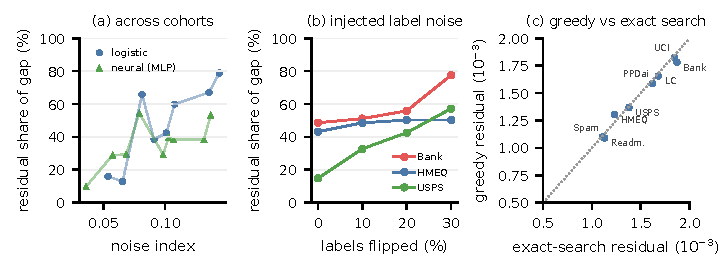
\includegraphics[width=\linewidth]{figures/fig_predict.pdf}
 \caption{(a) 基准 oracle 差距中的残差占比与标签噪声指数的关系，每个点对应一个数据集（表~\ref{tab:gradient}）。(b) 在数据集内随机翻转训练标签时的同一占比；每个剂量 16 个状态。(c) 12 候选池中贪心搜索与对全部可行集合精确搜索得到的残差，每个数据集 24 个状态；虚线为恒等线。}
 \label{fig:predict}
\end{figure}

\paragraph{预算越大下限越高；候选池更大则不一定。}把预算目标从 3 个调到 6 个再到 12 个低风险标签，八个数据集的族下限全部单调上升（均值 $0.67\to1.06\to1.41$；从 $k=3$ 到 $12$ 的配对增量为 $0.74$ $[0.67,0.82]$；图~\ref{fig:budget}），而可部署部分的变化远不一致。驱动上升的是获取的标签更多，而不是标签风险更大：所选集合的单标签结果方差几乎不变。这是经验规律而非定理，因为 $\Hpost$ 和 $\Hpre$ 都随预算变化。在固定预算下把候选池从 24 扩大到 48 再到 96，没有出现一致的规律（下限在 HMEQ 上上升，在银行营销和 USPS 上先升后降），因此我们不对候选池规模作任何断言。

\begin{figure}[t]
 \centering
 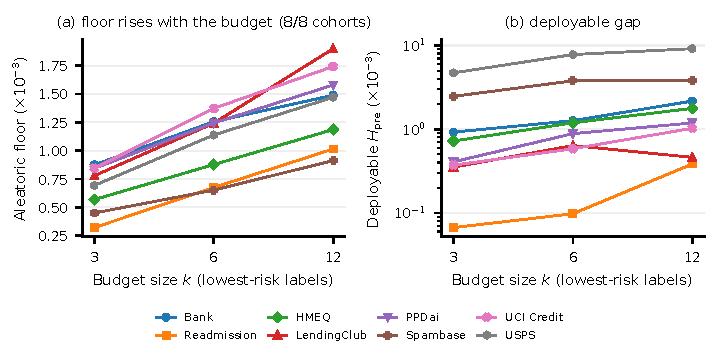
\includegraphics[width=\linewidth]{figures/fig_budget.pdf}
 \caption{风险预算作为调节杠杆（逻辑回归学习器，每个数据集、每个预算 32 个状态；预算按风险最低的 $k$ 个候选设定）。(a) 族下限在八个数据集上都随 $k$ 上升。(b) 可部署部分 $\Hpre$（交叉拟合，对数坐标）的变化远不一致。}
 \label{fig:budget}
\end{figure}

\paragraph{谁能弥合可部署部分取决于学习器。}表~\ref{tab:who} 在相同的真实标签状态上，把交叉拟合族收益与三种策略的收益作比较。使用逻辑回归学习器时，由逻辑回归模型导出的代理在可部署部分最大的地方弥合了其中很大一块：在工程流 HMEQ 和 LendingClub 上，TargetVar-greedy 和 Proxy-argmax 在 $3.2$--$3.4$ 中获得 $1.5$--$2.1$。使用提升学习器时，可部署部分仍有 $0.7$--$2.7$，但没有任何策略获得超过 $0.65$，DC-PRISM 的选择差距在八个信贷单元中有六个达到实质水平。信息代理只有在描述的正是将要训练的学习器时才有帮助。在再入院数据上，可部署部分很小（$0.7$--$0.9$），各策略之间没有决定性差异。

\begin{table}[t]
\caption{真实标签状态上的交叉拟合族收益与各策略相对 $M_K$ 的收益（每个单元信贷 64 个、再入院 128 个状态；$\times10^{-3}$ Brier）。DC：DC-PRISM；TV：TargetVar-greedy；Proxy：Proxy-argmax。}
\label{tab:who}
\centering\scriptsize
\setlength{\tabcolsep}{3pt}
\begin{tabular}{lrrrrrrrr}
\toprule
& \multicolumn{4}{c}{逻辑回归学习器} & \multicolumn{4}{c}{提升学习器} \\
\cmidrule(lr){2-5}\cmidrule(lr){6-9}
状态 & CF 收益 & DC & TV & Proxy & CF 收益 & DC & TV & Proxy \\
\midrule
HMEQ，工程 & 3.21 & 0.09 & 1.51 & 1.64 & 2.32 & 0.48 & 0.15 & 0.44 \\
LC，工程 & 3.37 & 1.15 & 2.01 & 2.12 & 1.53 & 0.05 & $-$0.42 & $-$0.19 \\
PPDai，工程 & 1.87 & 0.37 & 0.04 & 0.07 & 1.18 & 0.33 & 0.17 & 0.11 \\
UCI，工程 & 0.16 & $-$0.08 & $-$0.08 & $-$0.08 & 0.84 & 0.36 & 0.42 & 0.34 \\
HMEQ，自然 & 1.26 & $-$0.22 & 0.21 & 0.12 & 2.66 & 0.24 & 0.64 & 0.65 \\
LC，自然 & 0.91 & $-$0.04 & $-$0.20 & $-$0.05 & 1.45 & $-$0.07 & 0.04 & $-$0.04 \\
PPDai，自然 & 0.59 & 0.10 & $-$0.17 & 0.02 & 1.17 & $-$0.03 & $-$0.18 & $-$0.10 \\
UCI，自然 & 0.92 & 0.07 & 0.19 & 0.32 & 1.60 & 0.03 & 0.13 & 0.08 \\
再入院，工程 & 0.84 & 0.09 & $-$0.14 & $-$0.34 & 0.92 & $-$0.01 & $-$0.25 & $-$0.28 \\
再入院，自然 & 0.67 & 0.06 & 0.30 & 0.36 & 0.72 & 0.00 & $-$0.10 & $-$0.07 \\
\bottomrule
\end{tabular}
\end{table}

\paragraph{可部署部分较大时的 DC-PRISM。}在围绕方向性待回收信息构造的受控世界中，事后提升空间的 83\% 属于事前价值。DC-PRISM 相对 Safe-MinRisk 获得 $12.2$ $[7.6,16.8]$ 的收益，同时只获取 $3.1$ 个而不是 6 个标签；在我们尝试的全部十二种生成器变体中都保持实质水平（$10.8$--$31.4$；变化待回收重叠、风险--信息耦合、尾部误设，以及 48 个候选、$K=12$）。共同族消融把这一收益的大部分归于在锚定族上计算的代理（仅 Proxy-argmax 就获得 $13.1$ $[6.1,20.2]$）。保守层额外贡献的 $3.0$ $[-0.2,6.2]$ 未获证实，我们的证据也没有分离出待回收感知的贡献。

% ======================================================================
\section{结果检验：延迟回放}
\label{sec:replay}
协议对单轮打分。为检验它的诊断能否预测多轮结果，我们在延迟标签下回放十轮（探索标签一轮后到达，普通标签两轮后到达；ALC-Brier 为十个轮初分数的平均），每个信贷单元使用 512 个新种子，每个再入院流使用 256 个，样本量依据早先一批的方差设定。未被获取候选的标签只用于评价，因此这是一次全标签的回溯仿真，而不是选择性标签下的因果评估。表~\ref{tab:replay} 与单轮诊断相符。在信息贪心规则获得了可部署部分而 DC-PRISM 没有的地方（工程流 HMEQ 与 LendingClub），DC-PRISM 显著差于 Fisher-cost、BAIT-greedy 和 TargetVar-greedy，差距为 $2.5$--$3.8$。在其单轮相对数量基准的收益显著的地方，它以 $2.2$--$3.1$ 胜过 Safe-MinRisk 和固定数量。在工程流再入院上，它分别以 $1.3$ 和 $1.4$ 胜过 BAIT-greedy 和 TargetVar-greedy。在协议发现可部署价值很小的地方（自然流、工程流 UCI），没有任何比较达到实质水平：当下限主导 oracle 差距时，策略之间没有可争夺的东西。实现的不利敞口超过包络的情况，在每个信贷策略的 40{,}960 个获取轮次中至多 4 次，在再入院的 5{,}120 轮中为零。

\begin{table}[t]
\caption{延迟回放：对照策略减去 DC-PRISM 的 ALC-Brier（$\times10^{-3}$；正值有利于 DC-PRISM；粗体：在登记的比较族下达到实质水平）。}
\label{tab:replay}
\centering\scriptsize
\setlength{\tabcolsep}{2.4pt}
\begin{tabular}{lrrrrrrrrrr}
\toprule
& \multicolumn{4}{c}{信贷，工程流} & \multicolumn{4}{c}{信贷，自然流} & \multicolumn{2}{c}{再入院} \\
\cmidrule(lr){2-5}\cmidrule(lr){6-9}\cmidrule(lr){10-11}
对照策略 & HMEQ & LC & PPDai & UCI & HMEQ & LC & PPDai & UCI & 工程 & 自然 \\
\midrule
Safe-MinRisk & \textbf{2.4} & 0.4 & \textbf{3.1} & $-$0.1 & 0.2 & 0.2 & 0.4 & 0.1 & 0.0 & 0.2 \\
固定数量 & \textbf{2.2} & 0.4 & \textbf{2.4} & $-$0.1 & 0.1 & 0.1 & 0.3 & 0.0 & 0.4 & 0.2 \\
Random & 0.6 & $-$0.3 & \textbf{2.4} & 0.0 & 0.3 & 0.5 & 0.6 & 0.4 & 0.8 & 0.5 \\
Uncertainty & 0.5 & 1.4 & 0.7 & 0.0 & 0.4 & 0.4 & 0.1 & 0.1 & 0.4 & 0.0 \\
Fisher-cost & \textbf{$-$3.8} & \textbf{$-$3.3} & 0.8 & $-$0.1 & $-$0.3 & $-$0.1 & 0.1 & $-$0.1 & 1.0 & 0.0 \\
BAIT-greedy & \textbf{$-$3.6} & \textbf{$-$2.7} & 0.3 & 0.1 & $-$0.2 & 0.0 & 0.1 & 0.0 & \textbf{1.3} & 0.1 \\
TargetVar-greedy & \textbf{$-$3.5} & \textbf{$-$2.5} & 0.0 & 0.0 & $-$0.2 & $-$0.1 & 0.0 & $-$0.1 & \textbf{1.4} & 0.0 \\
\bottomrule
\end{tabular}
\end{table}

% ======================================================================
\section{相关工作}
\label{sec:related}
\paragraph{主动学习的评价。}主动学习的增益在贴近实际的评价下很脆弱~\cite{luth2023navigating}，对不受控的随机性敏感~\cite{ji2023randomness}，并且在不同领域间不一致~\cite{werner2023comparable,werner2024cdalbench}。oracle 被用来界定可达性能~\cite{werner2024cdalbench,huseljic2026boss}，Werner 等人也观察到他们的贪心 oracle 对测试集过拟合~\cite{werner2023comparable}。我们量化了这种复用，并识别出拆分测试集之后依然存在的第二个、偶然性的组成部分。

\paragraph{遗憾、信息价值与不确定性。}事前与事后遗憾在决策导向学习和鲁棒优化中有明确区分~\cite{schutte2023robust}；在 bandit 中，期望遗憾比伪遗憾多出一项噪声~\cite{bubeck2012regret,audibert2010regret}。完全信息价值是经典概念~\cite{howard1966information,raiffa1961applied}，从多个带噪估计中挑选最优者会带来乐观偏差~\cite{smith2006optimizer,cawley2010overfitting}。Brier 分数等严格适当评分规则允许区分偶然性与认知不确定性~\cite{hofman2024quantifying}。我们把这些思想迁移到标签获取的 oracle 上界，并让其中的偶然性部分能在真实数据上测量。

\paragraph{风险与延迟下的获取。}获取准则从不确定性与直推式设计，到 Fisher 信息、互信息、预测信息和决策损失~\cite{cohn1996active,settles2009active,lewis1994sequential,yu2006transductive,ash2021fishing,kirsch2019batchbald,bickfordsmith2023prediction,huang2026loss,chaloner1995bayesian}；预算与背包约束通常用贪心选择处理~\cite{krause2005near,sviridenko2004note,tomanek2010cost}。选择性标签~\cite{lakkaraju2017selective,wei2021selective,kilbertus2020fair,keswani2024partial,crook2004reject}、安全探索与安全主动学习~\cite{sui2015safe,schreiter2015safe,wu2016conservative}以及延迟反馈~\cite{joulani2013delayed,chapelle2014delayed,pham2022latency}构成了本文案例研究中风险约束设定的背景。

% ======================================================================
\section{结论}
\label{sec:conclusion}
在看到标签之后才做选择的 oracle，其收益有三个来源：复用评价集、所获标签中的结果运气，以及真正的事前信息。只有最后一项才是提升空间。在还款、再入院、认购这类记录随机结果的标签上，我们的研究中运气与复用构成了基准 oracle 领先的大部分；在手写数字这类近乎确定的标签上，领先大多是真实的。运气的占比在跨数据集比较和注入噪声时都随标签噪声上升，并随获取预算增大。我们建议 oracle 比较同时报告留出式 oracle 差距、下限估计、标签噪声水平以及下限对结果模型的敏感性。评判一个策略，应当以去掉运气和复用后剩下的那部分差距为准。

\paragraph{局限。}结果模型 $\hat p$ 不能识别真实的条件分布，我们的估计以固定测试集为条件；下限对 $\hat p$ 的离散程度最为敏感。残差只是近似等于族下限，精确搜索仅在 12 候选池中做过检验。标签翻转是受控干预，并不是自然不确定性的模型。候选池、学习器和预算的规模都有限；我们没有研究大型预训练模型或多分类标签。风险包络只有在条件独立且风险分数确为上界时才具有概率含义，而我们的经验分数不能保证这一点。各基线是其原始准则在风险预算下的改写版本。

\bibliographystyle{splncs04}
\bibliography{refs}
\end{document}
